\chapter{Bayesian Optimization}

Black box optimization of $f(x)$ where the evaluation is costly. Using GP as a
surrogate model. We use an \newterm{acquisition function} to find where the
next sample should be taken.

\section{Acquisition functions}

In each step, the objective function $f$ is sampled at $x_t = \argmax_x
u(x|D_{1:t-1})$ where $u$ is the acquisition function and $D_{1:t-1} =
((x_1,y_1),\ldots,(x_{t-1},y_{t-1}))$.

\begin{defn}
  \newterm{Expected improvement} $EI(x)$ is defined as

  \begin{equation}
    EI(x) = E_{Y \sim \gN(\mu, \sigma^2)} [max(f(x) - f(x^+), 0)]
  \end{equation}

  where $f(x^+)$ is the value of the best sample so far and $x^+ =
  \argmax_{x_i \in x_{1:t}} f(x_i)$.
\end{defn}

\section{Algorithm}

Iteratively for $t = 1,2,\ldots:$ {TODO NANDO}

\begin{itemize}
  \item Solve $x_t = \argmax_x u(x|D_{1:t-1})$ by combining the attributes of
    the posterior distribution in a utility function $u$.
  \item Sample the objective function $y_t = f(x_t) + \epsilon_t$.
  \item Augment the data $D_{1:t} = \set{D_{1:t-1}, (x_t, y_t)}$ and update
    the GP surrogate model based on the new data.
\end{itemize}


\subsection{Probability of Improvement}

We add a small term $\xi$ because otherwise $PI(x^+) = \frac{1}{2}.$

\begin{align}
  PI(x) &= P(f(x) \geq \mu^+ + \xi) \\
        &= \Phi \left(\frac{\mu(x) - \mu^+ - \xi}{\sigma(x)} \right)
\end{align}

where $\Phi$ is the CDF of a Gaussian. If we knew up front what is the best
value $f(x^*)$ we can model that directly by $P(f(x) \geq f(x^*))$.


\subsection{Expected utility}

At iteration $n+1$, choose the point that minimizes the distance to the
objective evaluated at the maximum $x^*$.

TODO undefined control sequence !

% \begin{align}
%   x_{n+1} &= \argmin_x E(\norm{\underbrace{f_{n+1}(x)}_{\text{GP}} - \underbrace{f(x^*)}_{\text{true}\ f} } | D_n) \\
%           &= \argmin_x \int \norm{f_{n+1}(x) - f(x^*)} p(f_{n+1} | D_n) \diff f_{n+1}
% \end{align}

We however don't know the true objective at the maximum. Instead we use (Mockus
et al., 1978 ??? TODO ref) where $f^{\max} = \mu^+ + \xi$

\begin{equation}
  x = \argmax_x E(\max\set{0, f_{n+1}(x) - f^{max}}|D_n)
\end{equation}

which can be solved analytically with

\begin{align}
  EI(x) &= \begin{cases}
    (\mu(x) - \mu^+ - \xi) \Phi(Z) + \sigma(x)\varphi(Z) & if \sigma(x) > 0 \\
    0 & if \sigma(x) = 0
  \end{cases} \\
  Z &= \frac{\mu(x) - \mu^+ - \xi}{\sigma(x)}
\end{align}

where $\phi(\cdot)$ and $\Phi(\cdot)$ denote the PDF and CDF of a normalized Gaussian.


\subsection{GP-UCB}

Define the \newterm{regret} and \newterm{cumulative regret} as follows:

\begin{align}
  r(x) &= f(x^*) - f(x) \\
  R_T &= r(x_1) + \cdots + r(x_T).
\end{align}

The GP-UCB criterion is as follows:

\begin{align}
  GP-UCB(x) = \mu(x) + \sqrt{\nu \beta} \sigma(x)
\end{align}

with $\nu = 1$ and $\beta_t = 2 \log(t^{d/2 + 2}\pi^2 / 3 \delta)$ where it can
be shown with high probability that this method has no regret, i.e. $\lim_{T
\rightarrow \infty} R_T / T = 0$. (Srinivas et at, 2010 TODO REF). (NOTE, if
the set of points is not infinite, $\beta$ ends up being different).


\subsection{Thompson sampling}

Draw a random sample (function) from the posterior, optimize to find its max,
evaluate the true $f(x)$ at the found max.

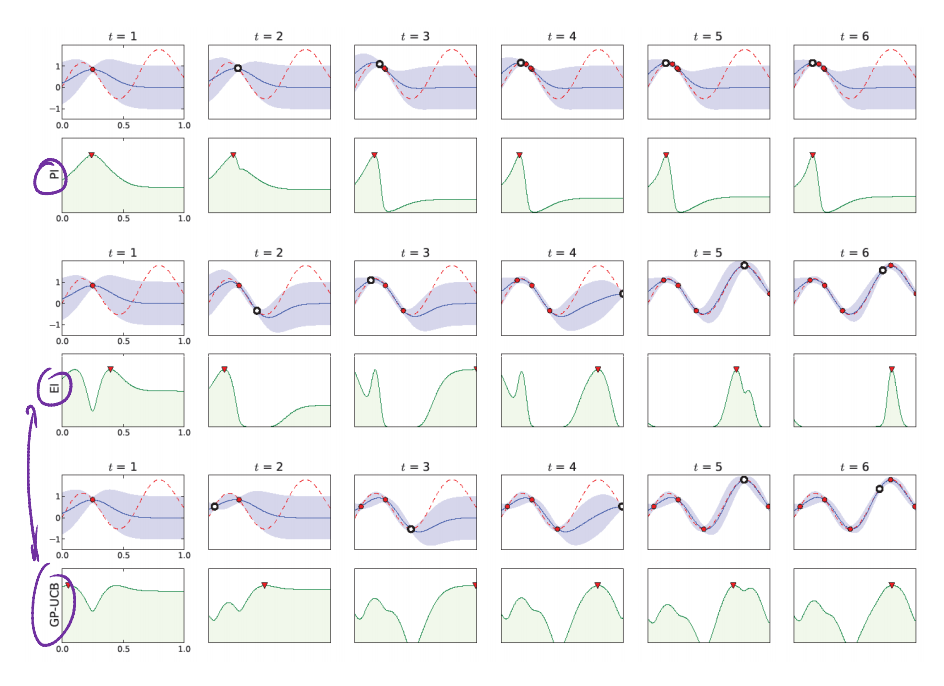
\includegraphics[width=0.9\textwidth]{img/acquisition-functions.png}

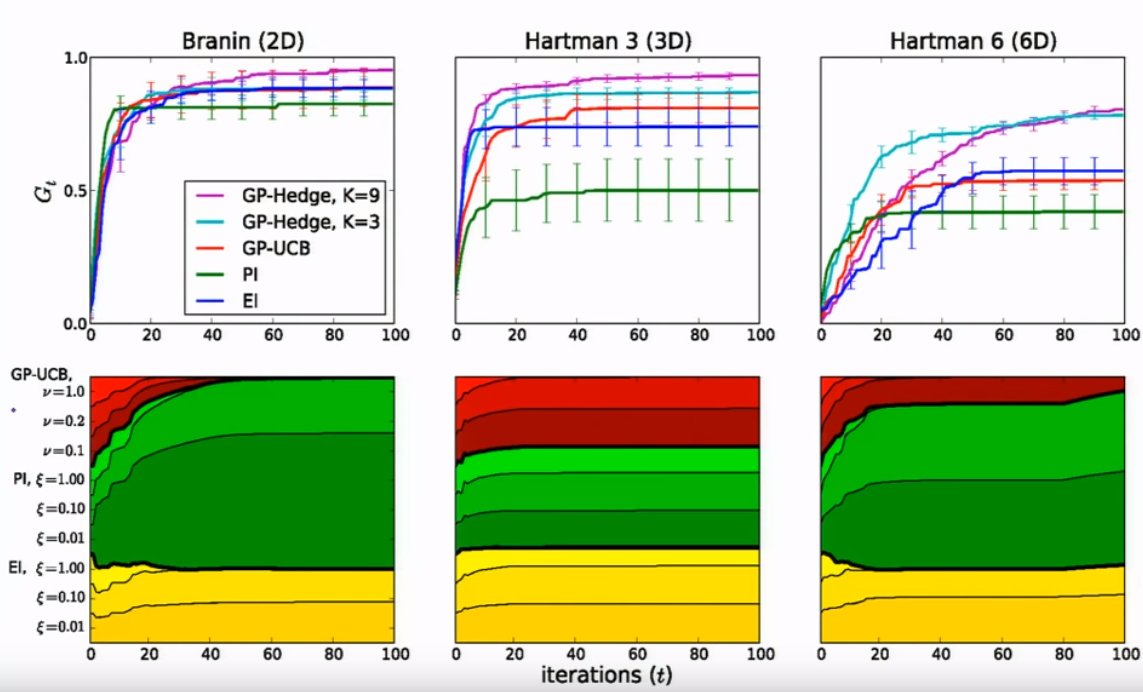
\includegraphics[width=0.9\textwidth]{img/portfolios-of-acquisition-functions.png}


\subsection{Max LCB}

There is no point in sampling where UCB is lower than $\max LCB$ (with high probability).
